\begin{figure}[ht!]
    \def\betaVar{3}
    \def\imgWidth{0.3\textwidth}
    \def\betaWidth{0.3\textwidth}
    \centering
    \begin{subfigure}{\betaWidth}
        \def\currentBeta{0}
        \centering
        \includegraphics[width=\imgWidth]{files/visualize_betas/beta_\currentBeta_-\betaVar_m}
        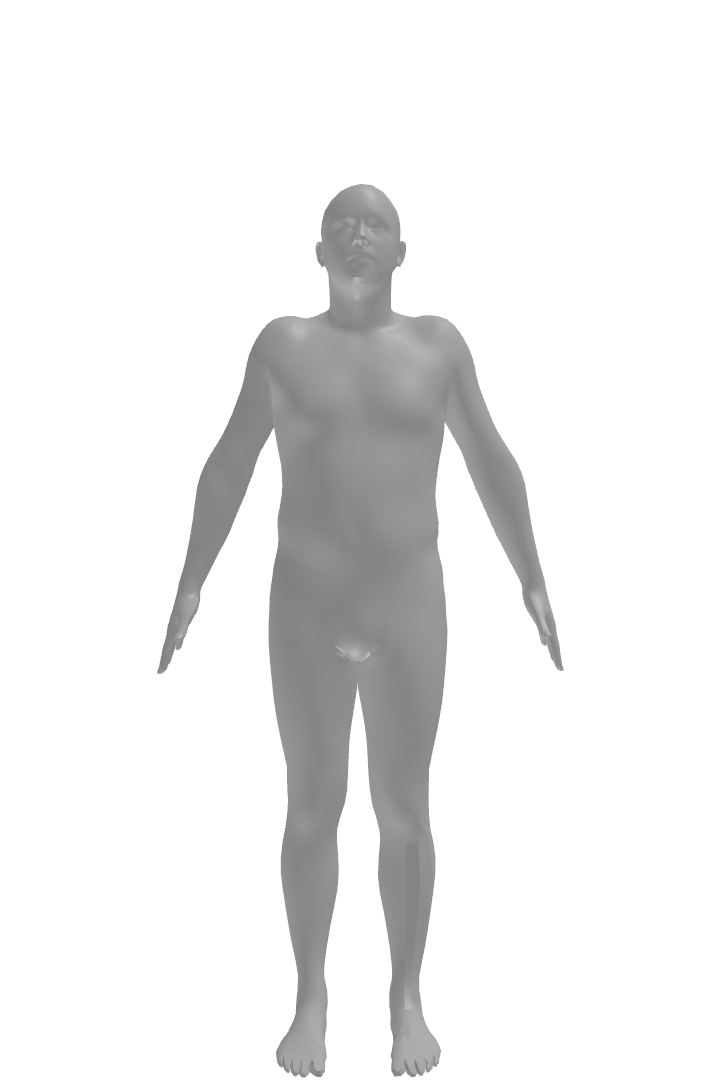
\includegraphics[width=\imgWidth]{files/visualize_betas/baseline_m}
        \includegraphics[width=\imgWidth]{files/visualize_betas/beta_\currentBeta_\betaVar_m}
        \linebreak
        \includegraphics[width=\imgWidth]{files/visualize_betas/beta_\currentBeta_-\betaVar_f}
        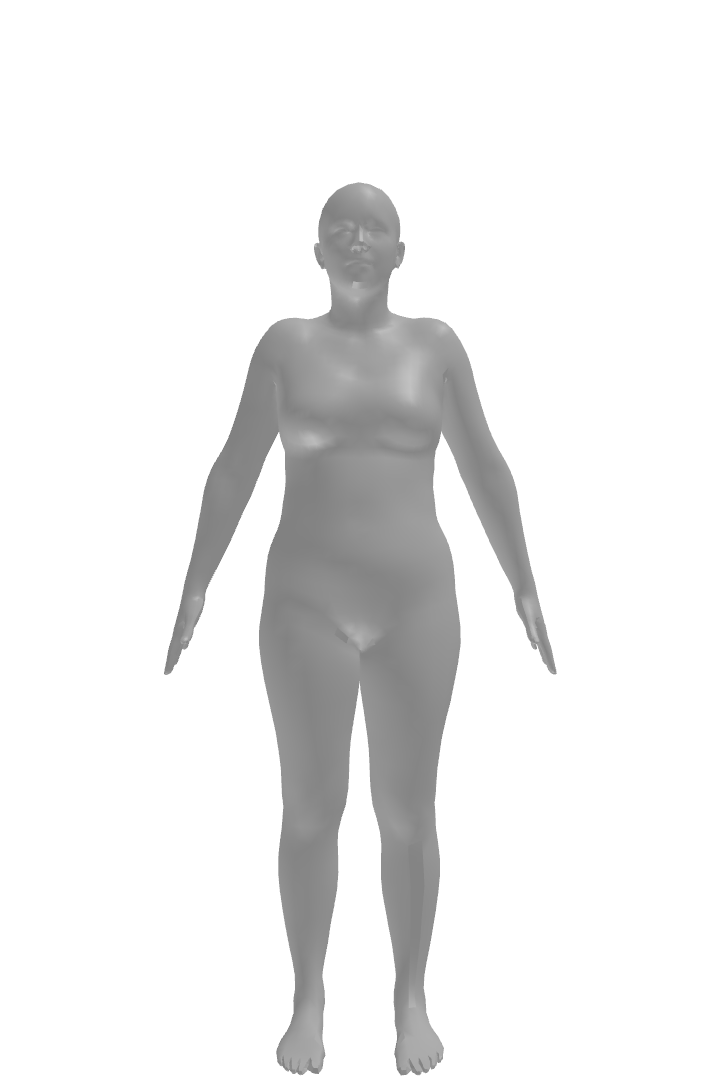
\includegraphics[width=\imgWidth]{files/visualize_betas/baseline_f}
        \includegraphics[width=\imgWidth]{files/visualize_betas/beta_\currentBeta_\betaVar_f}
        \caption{$\beta_1 = [-\betaVar, 0, +\betaVar]$}
    \end{subfigure}
    \begin{subfigure}{\betaWidth}
        \def\currentBeta{1}
        \centering
        \includegraphics[width=\imgWidth]{files/visualize_betas/beta_\currentBeta_-\betaVar_m}
        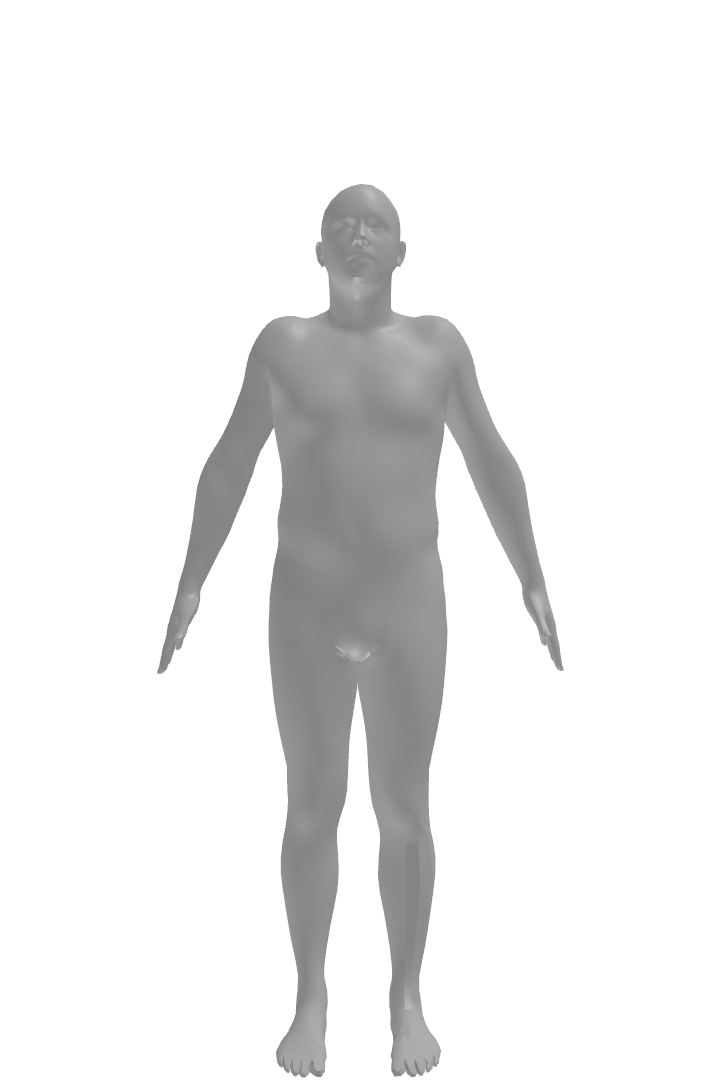
\includegraphics[width=\imgWidth]{files/visualize_betas/baseline_m}
        \includegraphics[width=\imgWidth]{files/visualize_betas/beta_\currentBeta_\betaVar_m}
        \linebreak
        \includegraphics[width=\imgWidth]{files/visualize_betas/beta_\currentBeta_-\betaVar_f}
        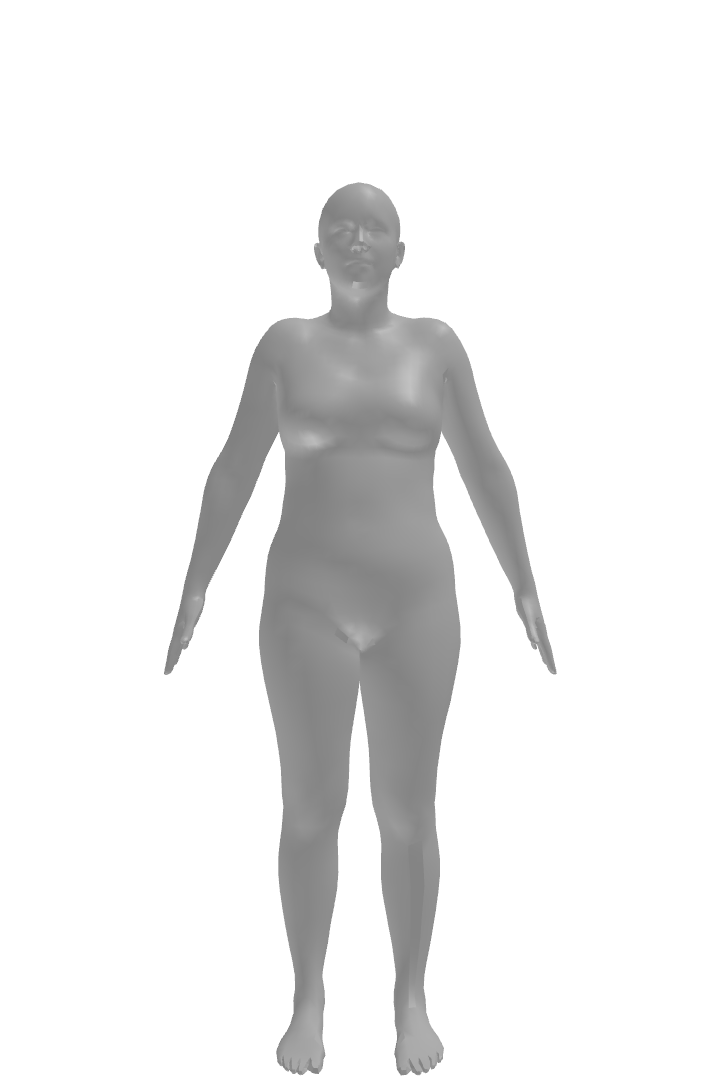
\includegraphics[width=\imgWidth]{files/visualize_betas/baseline_f}
        \includegraphics[width=\imgWidth]{files/visualize_betas/beta_\currentBeta_\betaVar_f}
        \caption{$\beta_2 = [-\betaVar, 0, +\betaVar]$}
    \end{subfigure}
    \begin{subfigure}{\betaWidth}
        \def\currentBeta{2}
        \centering
        \includegraphics[width=\imgWidth]{files/visualize_betas/beta_\currentBeta_-\betaVar_m}
        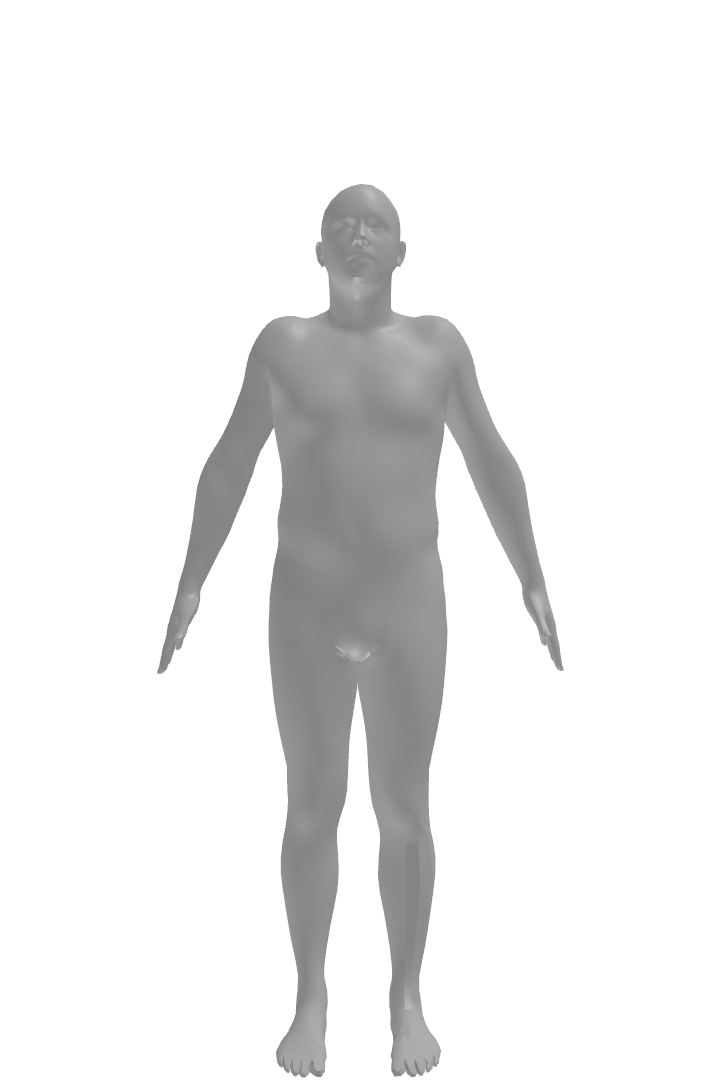
\includegraphics[width=\imgWidth]{files/visualize_betas/baseline_m}
        \includegraphics[width=\imgWidth]{files/visualize_betas/beta_\currentBeta_\betaVar_m}
        \linebreak
        \includegraphics[width=\imgWidth]{files/visualize_betas/beta_\currentBeta_-\betaVar_f}
        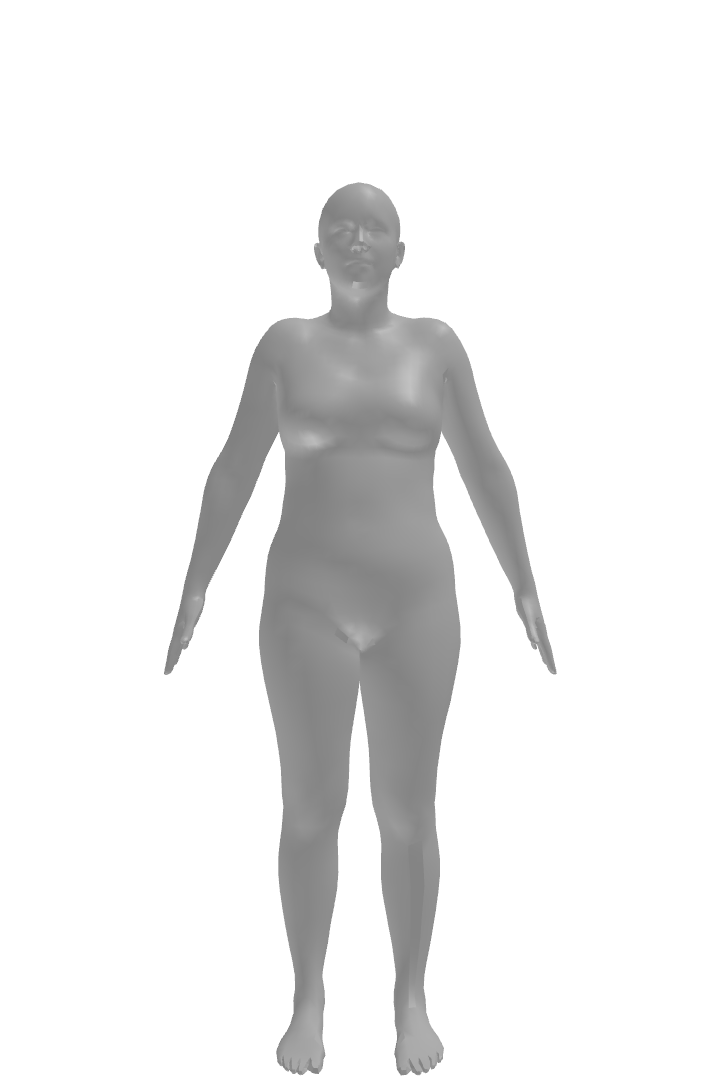
\includegraphics[width=\imgWidth]{files/visualize_betas/baseline_f}
        \includegraphics[width=\imgWidth]{files/visualize_betas/beta_\currentBeta_\betaVar_f}
        \caption{$\beta_3 = [-\betaVar, 0, +\betaVar]$}
    \end{subfigure}
    \begin{subfigure}{\betaWidth}
        \def\currentBeta{3}
        \centering
        \includegraphics[width=\imgWidth]{files/visualize_betas/beta_\currentBeta_-\betaVar_m}
        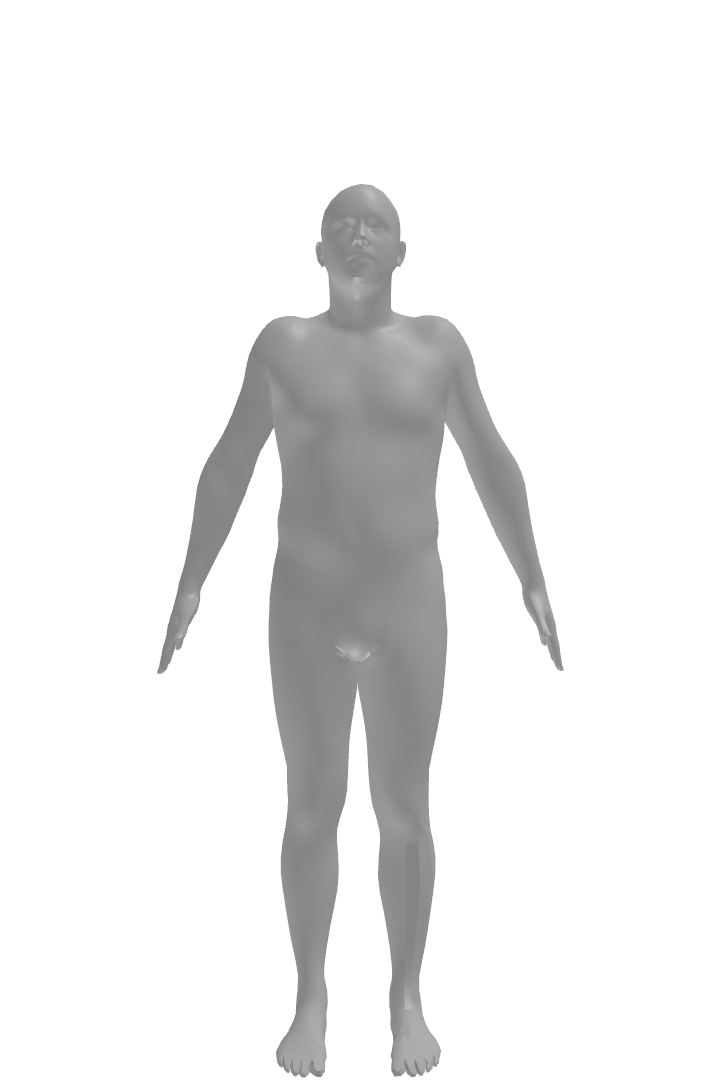
\includegraphics[width=\imgWidth]{files/visualize_betas/baseline_m}
        \includegraphics[width=\imgWidth]{files/visualize_betas/beta_\currentBeta_\betaVar_m}
        \linebreak
        \includegraphics[width=\imgWidth]{files/visualize_betas/beta_\currentBeta_-\betaVar_f}
        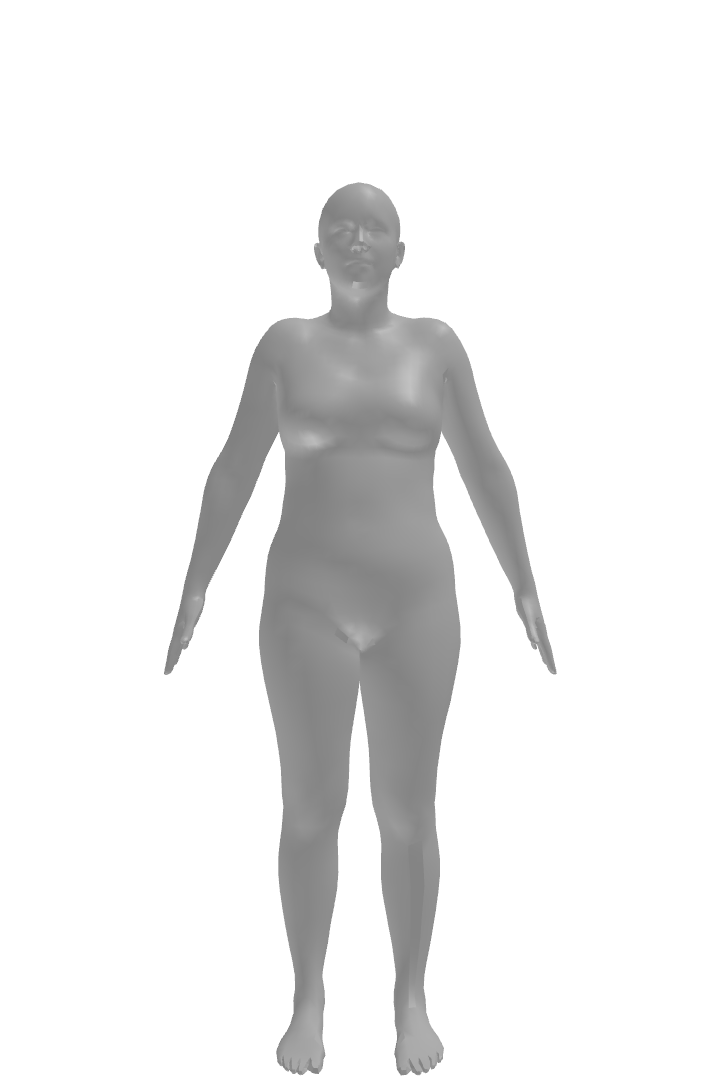
\includegraphics[width=\imgWidth]{files/visualize_betas/baseline_f}
        \includegraphics[width=\imgWidth]{files/visualize_betas/beta_\currentBeta_\betaVar_f}
        \caption{$\beta_4 = [-\betaVar, 0, +\betaVar]$}
    \end{subfigure}
    \begin{subfigure}{\betaWidth}
        \def\currentBeta{4}
        \centering
        \includegraphics[width=\imgWidth]{files/visualize_betas/beta_\currentBeta_-\betaVar_m}
        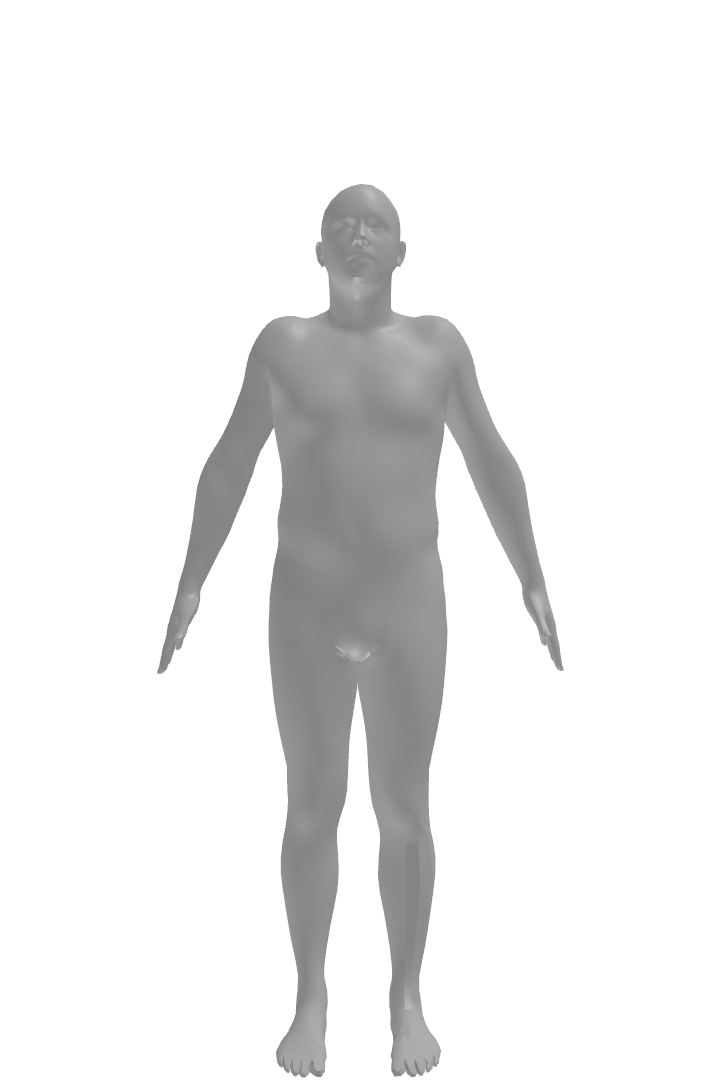
\includegraphics[width=\imgWidth]{files/visualize_betas/baseline_m}
        \includegraphics[width=\imgWidth]{files/visualize_betas/beta_\currentBeta_\betaVar_m}
        \linebreak
        \includegraphics[width=\imgWidth]{files/visualize_betas/beta_\currentBeta_-\betaVar_f}
        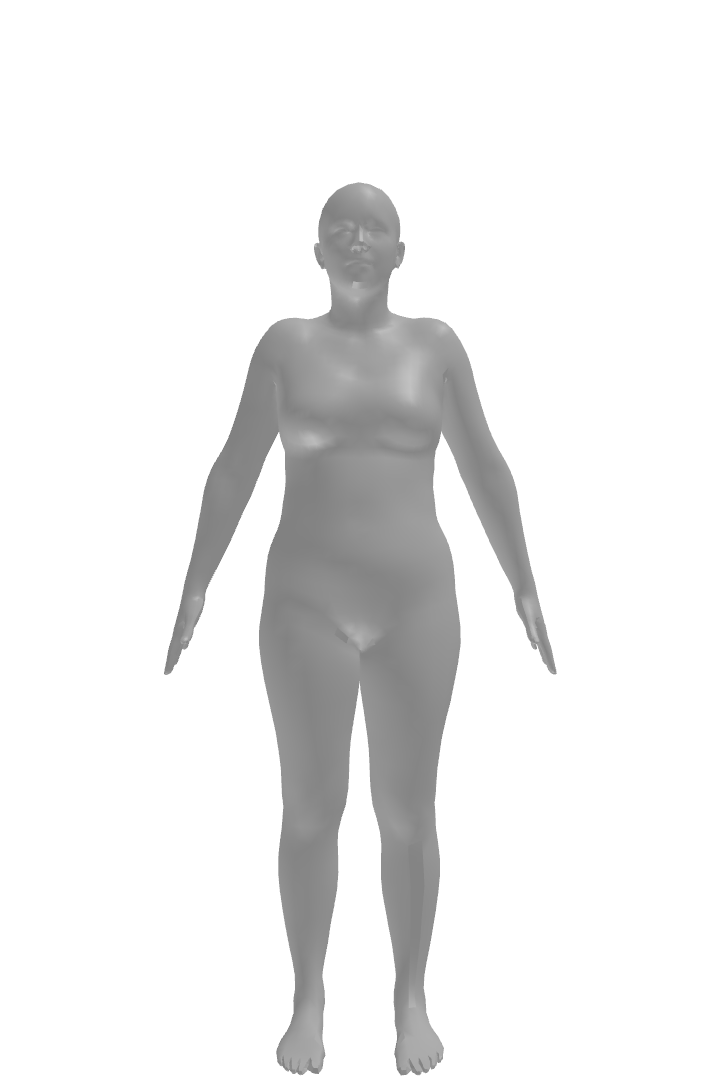
\includegraphics[width=\imgWidth]{files/visualize_betas/baseline_f}
        \includegraphics[width=\imgWidth]{files/visualize_betas/beta_\currentBeta_\betaVar_f}
        \caption{$\beta_5 = [-\betaVar, 0, +\betaVar]$}
    \end{subfigure}
    \begin{subfigure}{\betaWidth}
        \def\currentBeta{5}
        \centering
        \includegraphics[width=\imgWidth]{files/visualize_betas/beta_\currentBeta_-\betaVar_m}
        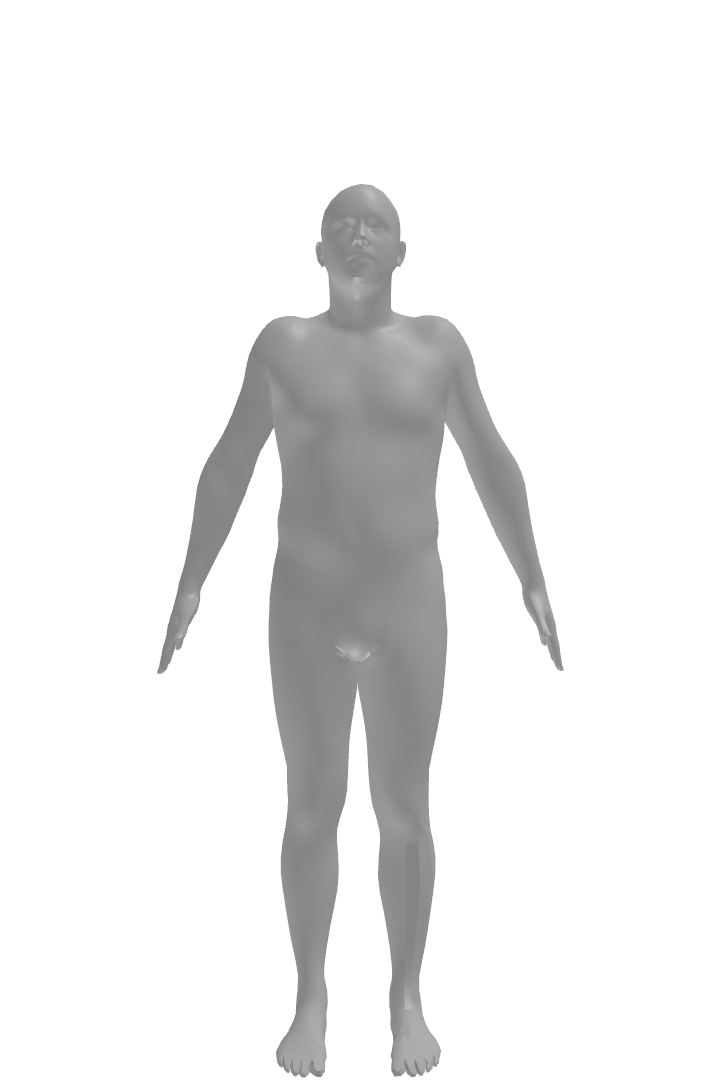
\includegraphics[width=\imgWidth]{files/visualize_betas/baseline_m}
        \includegraphics[width=\imgWidth]{files/visualize_betas/beta_\currentBeta_\betaVar_m}
        \linebreak
        \includegraphics[width=\imgWidth]{files/visualize_betas/beta_\currentBeta_-\betaVar_f}
        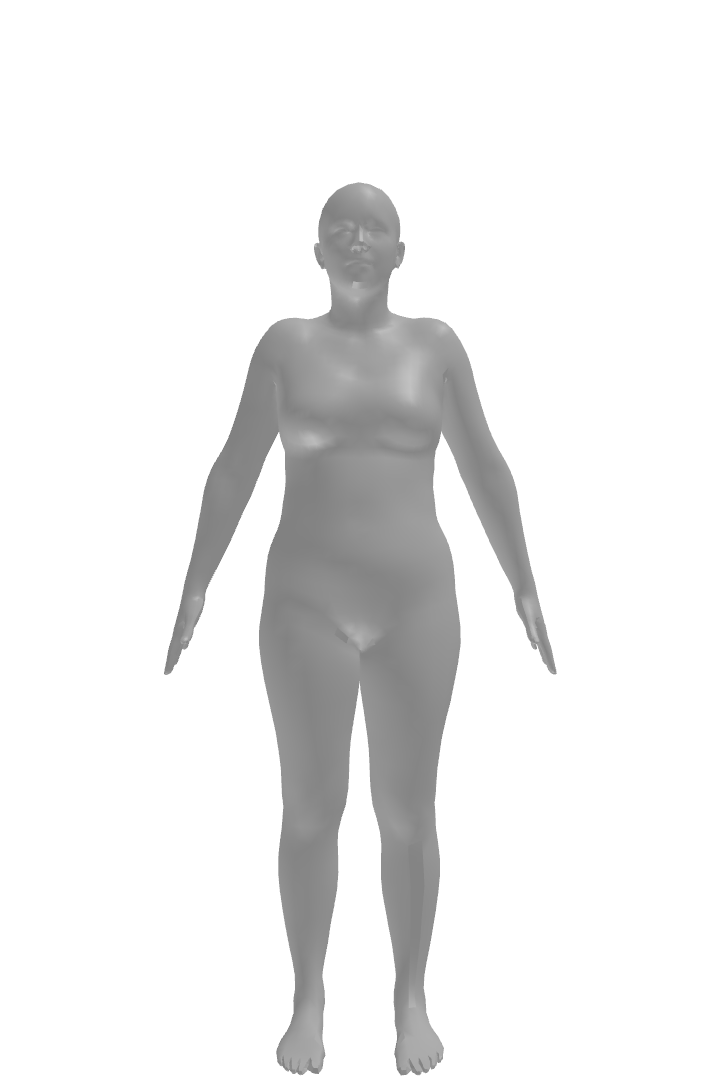
\includegraphics[width=\imgWidth]{files/visualize_betas/baseline_f}
        \includegraphics[width=\imgWidth]{files/visualize_betas/beta_\currentBeta_\betaVar_f}
        \caption{$\beta_6 = [-\betaVar, 0, +\betaVar]$}
    \end{subfigure}
    \begin{subfigure}{\betaWidth}
        \def\currentBeta{6}
        \centering
        \includegraphics[width=\imgWidth]{files/visualize_betas/beta_\currentBeta_-\betaVar_m}
        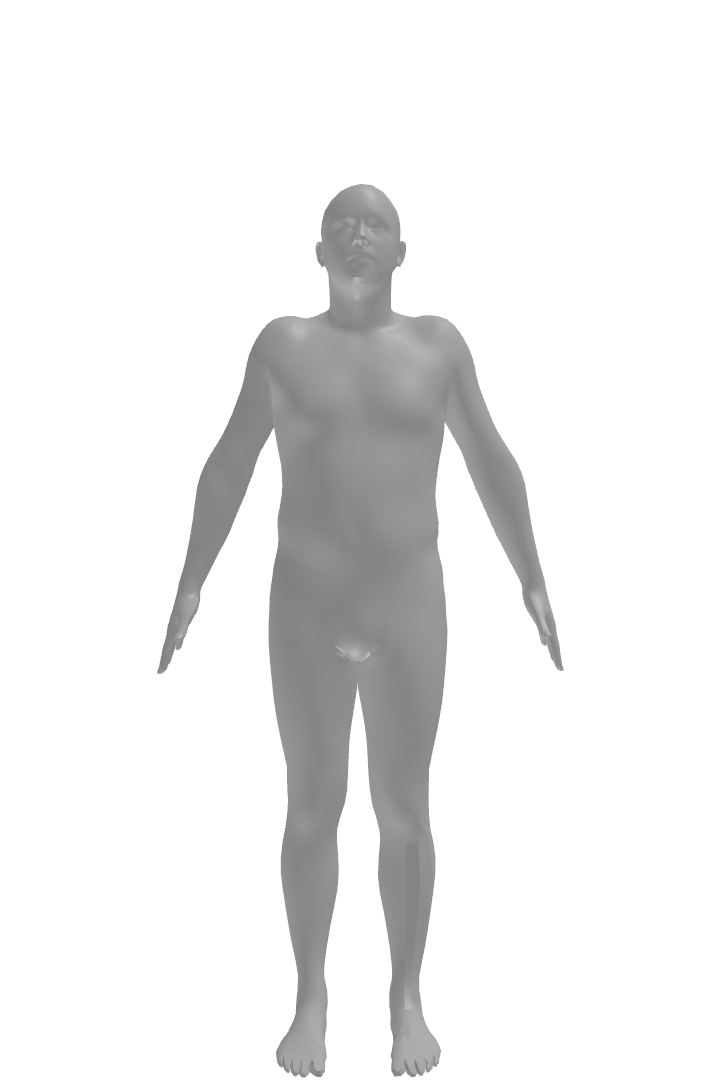
\includegraphics[width=\imgWidth]{files/visualize_betas/baseline_m}
        \includegraphics[width=\imgWidth]{files/visualize_betas/beta_\currentBeta_\betaVar_m}
        \linebreak
        \includegraphics[width=\imgWidth]{files/visualize_betas/beta_\currentBeta_-\betaVar_f}
        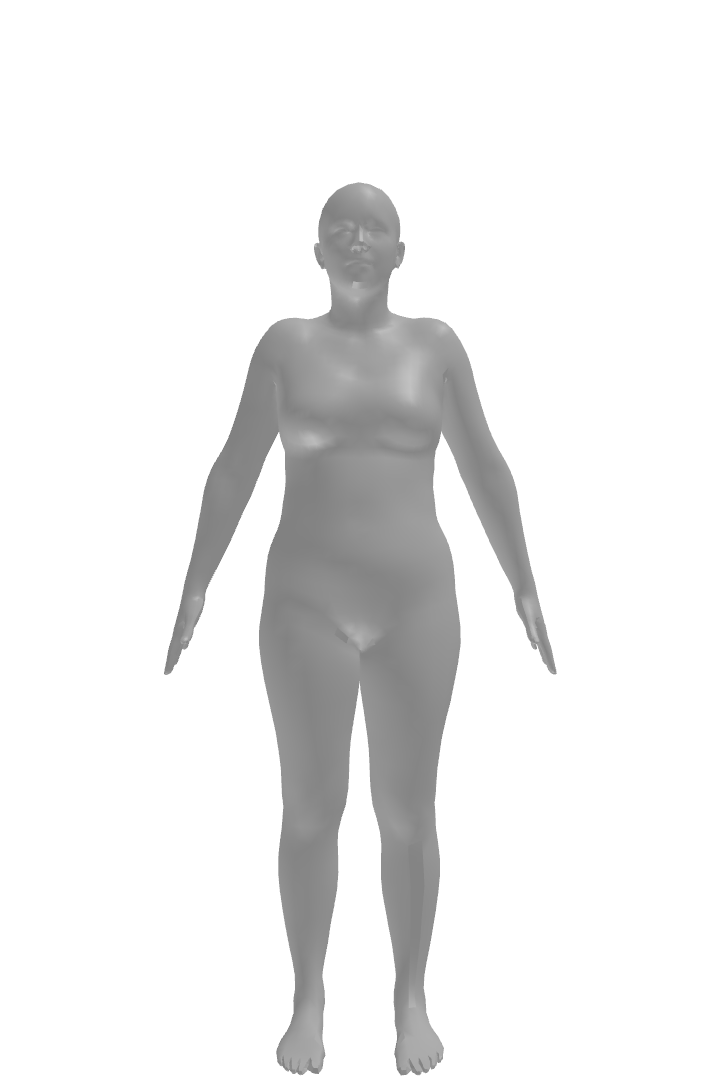
\includegraphics[width=\imgWidth]{files/visualize_betas/baseline_f}
        \includegraphics[width=\imgWidth]{files/visualize_betas/beta_\currentBeta_\betaVar_f}
        \caption{$\beta_7 = [-\betaVar, 0, +\betaVar]$}
    \end{subfigure}
    \begin{subfigure}{\betaWidth}
        \def\currentBeta{7}
        \centering
        \includegraphics[width=\imgWidth]{files/visualize_betas/beta_\currentBeta_-\betaVar_m}
        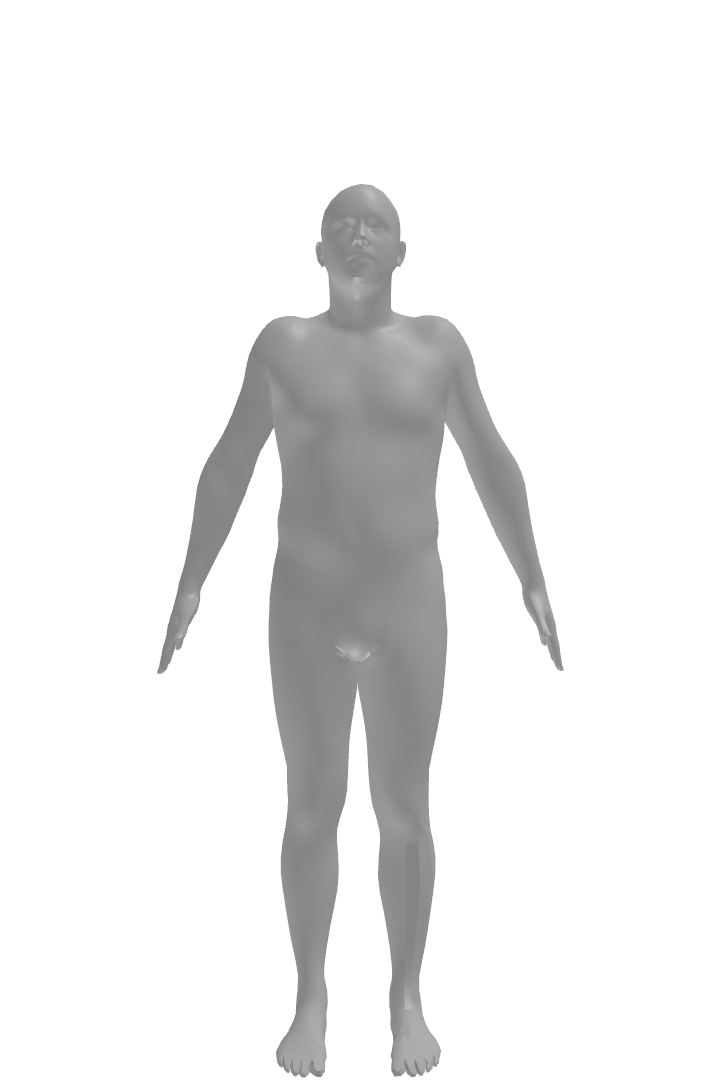
\includegraphics[width=\imgWidth]{files/visualize_betas/baseline_m}
        \includegraphics[width=\imgWidth]{files/visualize_betas/beta_\currentBeta_\betaVar_m}
        \linebreak
        \includegraphics[width=\imgWidth]{files/visualize_betas/beta_\currentBeta_-\betaVar_f}
        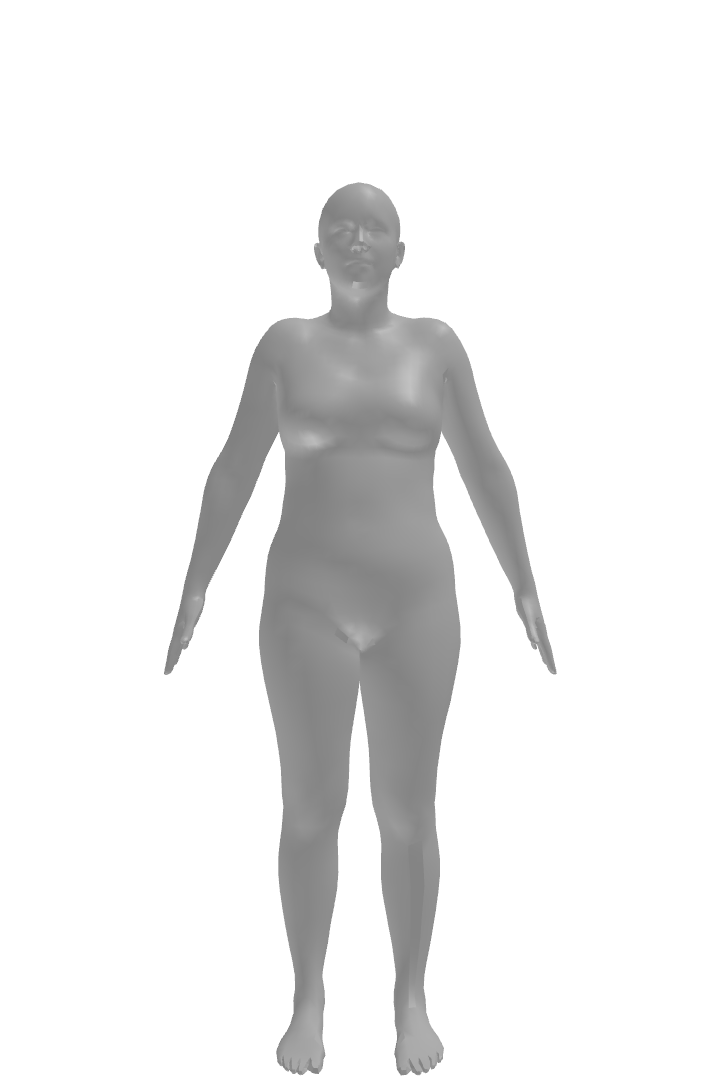
\includegraphics[width=\imgWidth]{files/visualize_betas/baseline_f}
        \includegraphics[width=\imgWidth]{files/visualize_betas/beta_\currentBeta_\betaVar_f}
        \caption{$\beta_8 = [-\betaVar, 0, +\betaVar]$}
    \end{subfigure}
    \begin{subfigure}{\betaWidth}
        \def\currentBeta{8}
        \centering
        \includegraphics[width=\imgWidth]{files/visualize_betas/beta_\currentBeta_-\betaVar_m}
        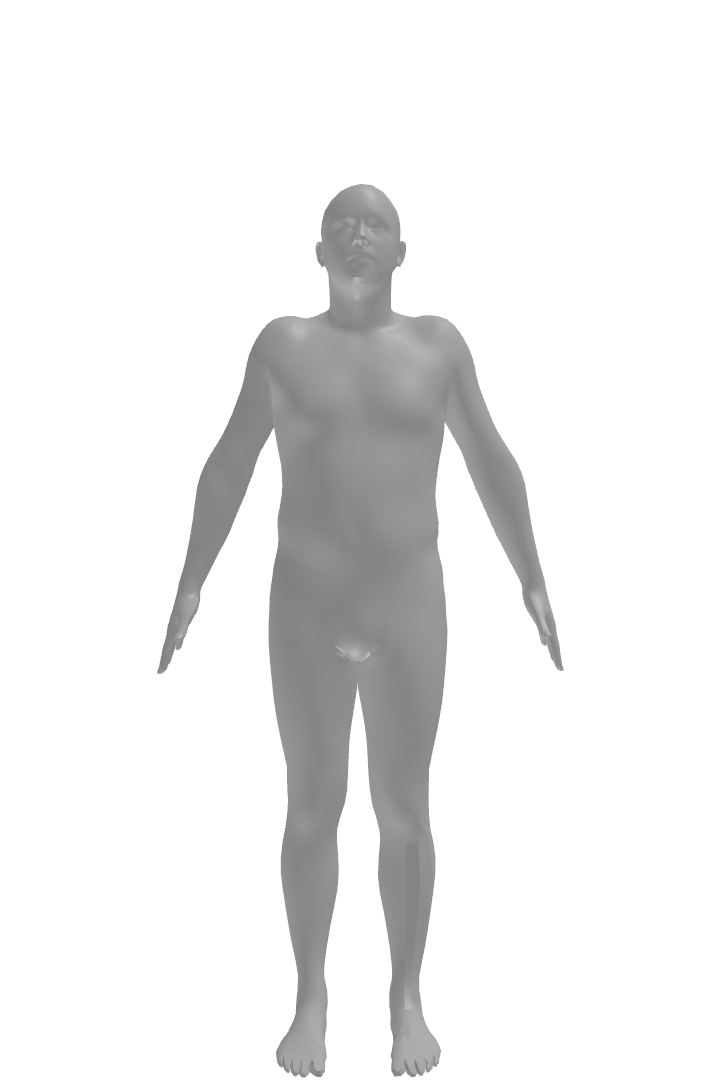
\includegraphics[width=\imgWidth]{files/visualize_betas/baseline_m}
        \includegraphics[width=\imgWidth]{files/visualize_betas/beta_\currentBeta_\betaVar_m}
        \linebreak
        \includegraphics[width=\imgWidth]{files/visualize_betas/beta_\currentBeta_-\betaVar_f}
        \includegraphics[width=\imgWidth]{files/visualize_betas/baseline_f}
        \includegraphics[width=\imgWidth]{files/visualize_betas/beta_\currentBeta_\betaVar_f}
        \caption{$\beta_9 = [-\betaVar, 0, +\betaVar]$}
    \end{subfigure}
    \begin{subfigure}{\betaWidth}
        \def\currentBeta{9}
        \centering
        \includegraphics[width=\imgWidth]{files/visualize_betas/beta_\currentBeta_-\betaVar_m}
        \includegraphics[width=\imgWidth]{files/visualize_betas/baseline_m}
        \includegraphics[width=\imgWidth]{files/visualize_betas/beta_\currentBeta_\betaVar_m}
        \linebreak
        \includegraphics[width=\imgWidth]{files/visualize_betas/beta_\currentBeta_-\betaVar_f}
        \includegraphics[width=\imgWidth]{files/visualize_betas/baseline_f}
        \includegraphics[width=\imgWidth]{files/visualize_betas/beta_\currentBeta_\betaVar_f}
        \caption{$\beta_{10} = [-\betaVar, 0, +\betaVar]$}
    \end{subfigure}
    \caption{Visual representation of what the \gls{smpl} shape parameters represent for
        male and female bodies}\label{fig:beta-vis}
\end{figure}